\documentclass[11pt,a4paper]{article}
\usepackage[utf8]{inputenc}
\usepackage[T1]{fontenc}
\usepackage[catalan]{babel}
\usepackage{amsmath,amssymb}
\usepackage{array}
\usepackage{graphicx}
\usepackage{booktabs}
\usepackage{float}
\usepackage{caption}
\usepackage{subcaption}
\usepackage{xcolor}
\usepackage{enumitem}
\usepackage{indentfirst}   % indenta també el primer paràgraf de cada secció
\usepackage{titlesec}
\usepackage[margin=2.5cm]{geometry}
\usepackage[colorlinks=true,linkcolor=blue!50!black,citecolor=blue!50!black,urlcolor=blue!50!black]{hyperref}

% --- Format ---------------------------------------------------------------
\setlength{\parindent}{1.5em}          % sagnia de paràgraf
\setlength{\parskip}{0pt}
\titleformat{\section}{\large\bfseries}{\thesection}{0.7em}{}   % títols amb només la 1a lletra en majúscula
\titlespacing*{\section}{0pt}{0pt}{0.25cm}                      % l'espai de 0,4 cm es posa amb \vspace abans de cada \section
\setlist[itemize]{label=-, leftmargin=1.5em, itemsep=1pt, topsep=3pt}
\setlist[enumerate]{leftmargin=1.5em, itemsep=1pt, topsep=3pt}
\captionsetup{font=small, labelfont=bf, skip=4pt}
\setlength{\textfloatsep}{10pt plus 2pt minus 2pt}

\title{Identificació de mòduls de gens co-expressats i validació sense etiquetes en dades d'expressió gènica mitjançant aprenentatge no supervisat}
\author{Martí Canut Sumarroca\\ \small Grup: Matías, Martí, Uriel i Arnau}
\date{\today}

\begin{document}
\maketitle

\begin{abstract}
Aquesta implementació aplica l'aprenentatge no supervisat al conjunt de dades de leucèmia de Golub et al.\ (72 pacients, 7.129 gens) per comprovar, primer, si és possible recuperar sense etiquetes la distinció entre leucèmia limfoblàstica aguda (ALL) i mieloide aguda (AML) i, segon, quins grups de gens mostren patrons d'expressió semblants. Després d'un preprocessament logarítmic i d'una selecció dels 500 gens més variables, s'agrupen els pacients amb clustering jeràrquic (tres tipus d'enllaç) i K-Means, i els gens amb clustering jeràrquic de distància de correlació. Els diagnòstics clínics s'usen només per validar els models. K-Means assoleix un ARI de 0,89 i l'enllaç \emph{complete} de 0,79, mentre que el coeficient de Silhouette indica $k=2$ com a nombre òptim de grups.
\end{abstract}

%====================================================================
\vspace{0.4cm}
\section{Plantejament del problema}

Les cèl·lules fabriquen proteïnes a partir de la informació dels gens, i ho fan a través de l'ARN missatger (mRNA): com més activitat té un gen, més mRNA se'n detecta. Aquesta quantitat s'anomena \emph{nivell d'expressió}. Tècniques com el microarray d'oligonucleòtids (usat a~\cite{golub}) o la seqüenciació d'ARN la mesuren per a milers de gens alhora, de manera que cada pacient queda descrit per un vector amb els nivells d'expressió de tots els gens mesurats. Les leucèmies agudes limfoblàstica (ALL) i mieloide (AML) deriven de línies cel·lulars diferents de la sang i requereixen tractaments diferents; per això distingir-les bé és clínicament rellevant.

El problema és naturalment no supervisat per dos motius. Primer, no sabem a priori quins gens funcionen junts: els gens que s'expressen amb patrons semblants entre pacients (gens co-expressats) sovint estan regulats conjuntament o participen en processos biològics comuns~\cite{eisen}, però aquesta informació no ve etiquetada. Segon, volem comprovar si l'estructura de les dades, per si sola, reprodueix el diagnòstic clínic sense haver-lo vist durant el modelatge. A més, es treballa amb alta dimensionalitat (7.129 gens per només 72 pacients), una situació on les distàncies són poc intuïtives i cal escollir amb cura la mètrica i el preprocessament.

Els objectius de la implementació són els següents:
\begin{enumerate}
  \item Identificar les leucèmies ALL/AML sense etiquetes, tallant l'arbre o K-Means a $k=2$, amb un ARI superior a 0,7.
  \item Comparar tres criteris d'enllaç (\emph{single}, \emph{complete}, \emph{average}) i K-Means, amb una mètrica interna (Silhouette) i una d'externa (ARI).
  \item Identificar mòduls de gens co-expressats i triar-ne el nombre amb el coeficient de Silhouette.
  \item Visualitzar conjuntament gens i pacients amb un mapa de calor (via dendrogrames).
\end{enumerate}
Pel que fa a l'abast i els supòsits, s'usa un únic conjunt de dades, es treballa amb els 500 gens més variables, la distància és de correlació (o euclidiana), les etiquetes ALL/AML només s'usen després del clustering per validar, no s'elimina cap pacient i no s'interpreten biològicament els mòduls de gens.

Com a aportacions pròpies, el treball agrupa tant pacients com gens i els mostra junts, compara el mapa de calor brut amb el reordenat pels dendrogrames per veure què aporta el clustering, i corregeix un problema de preprocessament detectat en una primera versió (apartat de Metodologia).

%====================================================================
\vspace{0.4cm}
\section{Fonament teòric}

Per comparar perfils d'expressió interessa la \emph{forma} del patró i no la seva magnitud: dos gens que pugen i baixen igual entre pacients han de ser veïns encara que un tingui el doble d'amplitud. Per això s'usa la distància de correlació de Pearson, $d_r(u,v)=1-r(u,v)$, que val 0 si els perfils estan perfectament correlacionats i 2 si estan perfectament anticorrelacionats; combinada amb l'enllaç \emph{average}, és l'opció clàssica en expressió gènica~\cite{eisen}. K-Means, en canvi, usa la distància euclidiana.

El clustering jeràrquic aglomeratiu parteix de cada element com a clúster propi i fusiona a cada pas els dos clústers més propers; el resultat és un arbre (dendrograma) que es pot tallar a l'altura desitjada per obtenir $k$ grups. Els criteris d'enllaç difereixen en com mesuren la distància entre clústers:
\begin{itemize}
  \item \textbf{Single:} distància mínima entre parells d'elements (sensible a punts aïllats i a l'efecte cadena).
  \item \textbf{Complete:} distància màxima entre parells; afavoreix clústers compactes.
  \item \textbf{Average:} distància mitjana entre tots els parells; equilibri entre els dos anteriors.
\end{itemize}
K-Means divideix les dades en $k$ grups minimitzant la \emph{inèrcia}, és a dir, la suma de quadrats de les distàncies de cada punt al centre del seu grup. Cal fixar $k$ per endavant i el resultat depèn de la inicialització, per això es repeteix diverses vegades i es guarda la millor. El \emph{mètode del colze} representa la inèrcia en funció de $k$ i busca el punt on la millora deixa de ser apreciable.

Per validar sense etiquetes s'usa el \emph{coeficient de Silhouette}~\cite{rousseeuw}, que mesura com de bé encaixa cada element $i$ en el seu grup, $s(i)=\frac{b(i)-a(i)}{\max\{a(i),b(i)\}}\in[-1,1]$, on $a(i)$ és la distància mitjana als altres elements del seu grup i $b(i)$ la del grup veí més proper; se'n tria el $k$ de silueta mitjana màxima. Com a validació externa s'usa l'\emph{Adjusted Rand Index} (ARI)~\cite{hubert}, que compara dues particions comptant els parells d'elements que coincideixen i corregeix l'acord esperat per atzar: val 1 si són idèntiques, aproximadament 0 si equivalen a una partició aleatòria i pot ser lleugerament negatiu. Les fórmules completes són a l'Annex~\ref{ann:formules}.

Finalment, un \emph{clustermap} mostra la matriu d'expressió com un mapa de calor amb files (gens) i columnes (pacients) reordenades segons els seus dendrogrames, de manera que els blocs de color revelen gens co-expressats en grups de pacients~\cite{eisen}.

%====================================================================
\vspace{0.4cm}
\section{Metodologia}

\textbf{Dades.} S'ha utilitzat el conjunt de Golub et al.~\cite{golub}, descarregat d'OpenML (ID 1104): l'expressió de 7.129 gens, mesurada amb microarrays Affymetrix, en 72 pacients (47 ALL i 25 AML), organitzada en una matriu $X\in\mathbb{R}^{7129\times 72}$. Les etiquetes clíniques no intervenen en cap etapa del modelatge. La matriu en brut no té valors nuls, va de $-28.400$ a $71.369$ i és molt asimètrica (mitjana 619,78, mediana 120,00); els valors negatius provenen de la correcció del fons i no tenen sentit com a expressió.

\textbf{Preprocessament.} S'inspira en el de Golub et al.~\cite{golub}. Primer, un retall de rang a $[100,\,16.000]$ (\texttt{np.clip}), que elimina els valors negatius i les fluctuacions per sota del límit de detecció i limita la saturació dels detectors. Després, la transformació $x'=\log_2(x+1)$, que redueix l'asimetria, estabilitza la variància i fa que les diferències es llegeixin com a canvis relatius d'expressió (\emph{fold-change}); com que $x\ge100$, el $+1$ és innecessari però inofensiu. Una primera versió retallava només a 0: concentrava més de $10^5$ valors en un sol punt i feia aparèixer gens amb variàncies artificialment altes, que haurien dominat la selecció posterior. Finalment, es conserven els $N=500$ gens de variància més alta, perquè els gens gairebé constants no informen sobre diferències entre pacients (selecció sense etiquetes), i cada gen s'estandarditza amb el z-score, $z=(x-\mu)/\sigma$ entre pacients. El resultat és una matriu $X_{\text{clean}}\in\mathbb{R}^{500\times72}$.

\textbf{Clustering dels pacients.} S'agrupen els 72 pacients, cadascun descrit pels seus 500 gens, amb distància de correlació i tres criteris d'enllaç (\emph{single}, \emph{complete} i \emph{average}). Per a cada enllaç es talla l'arbre a $k=2$ i es calcula l'ARI contra el diagnòstic. El dendrograma i el clustermap es fan amb \emph{average}, que s'ha fixat des del principi (no pas mirant l'ARI) perquè és l'opció estàndard amb distància de correlació en expressió gènica~\cite{eisen}. Amb K-Means es fa servir $k=2,\dots,8$, amb 10 inicialitzacions i llavor fixa; per a cada $k$ es guarden la inèrcia i la silueta mitjana, i per a $k=2$ l'ARI.

\textbf{Mòduls de gens i mapes de calor.} S'agrupen els 500 gens, cadascun descrit pels seus valors en els 72 pacients, amb distància de correlació i enllaç \emph{average}. Per a $k=2,\dots,10$ es talla l'arbre, es calcula la silueta amb la matriu de distàncies precalculada i es tria el $k$ de silueta màxima, que defineix el mòdul de cada gen. Després es representa $X_{\text{clean}}$ en dues versions: sense reordenar (ordre original dels pacients i ordre de selecció dels gens) i reordenada pels dos dendrogrames (clustermap), amb barres de color pel diagnòstic i pel mòdul. Comparar-les mostra què aporta el clustering.

\textbf{Implementació.} El codi és en Python: NumPy i pandas per a les dades, SciPy per al clustering jeràrquic, scikit-learn~\cite{sklearn} per a K-Means, la silueta i l'ARI, i Matplotlib i seaborn per als gràfics. Cada pas és una funció amb \emph{docstring}, totes les llavors són fixes i el repositori inclou un \texttt{README} i un \texttt{requirements.txt}; totes les figures i xifres d'aquest informe s'obtenen d'una única execució del programa.

%====================================================================
\vspace{0.4cm}
\section{Resultats i anàlisi}

La Figura~\ref{fig:hist} mostra l'efecte del retall i del logaritme: la distribució original, molt asimètrica i amb valors negatius, queda acotada entre $\log_2(101)\approx6{,}66$ i $\log_2(16001)\approx13{,}97$. Els dos pics extrems corresponen als valors retallats (47,0\,\% al terra i 0,8\,\% al sostre), una limitació del retall perquè tots els gens poc expressats queden al mateix valor. El filtre per variància conserva els 500 gens amb variància $\ge1{,}30$.

\begin{figure}[!htb]
\centering
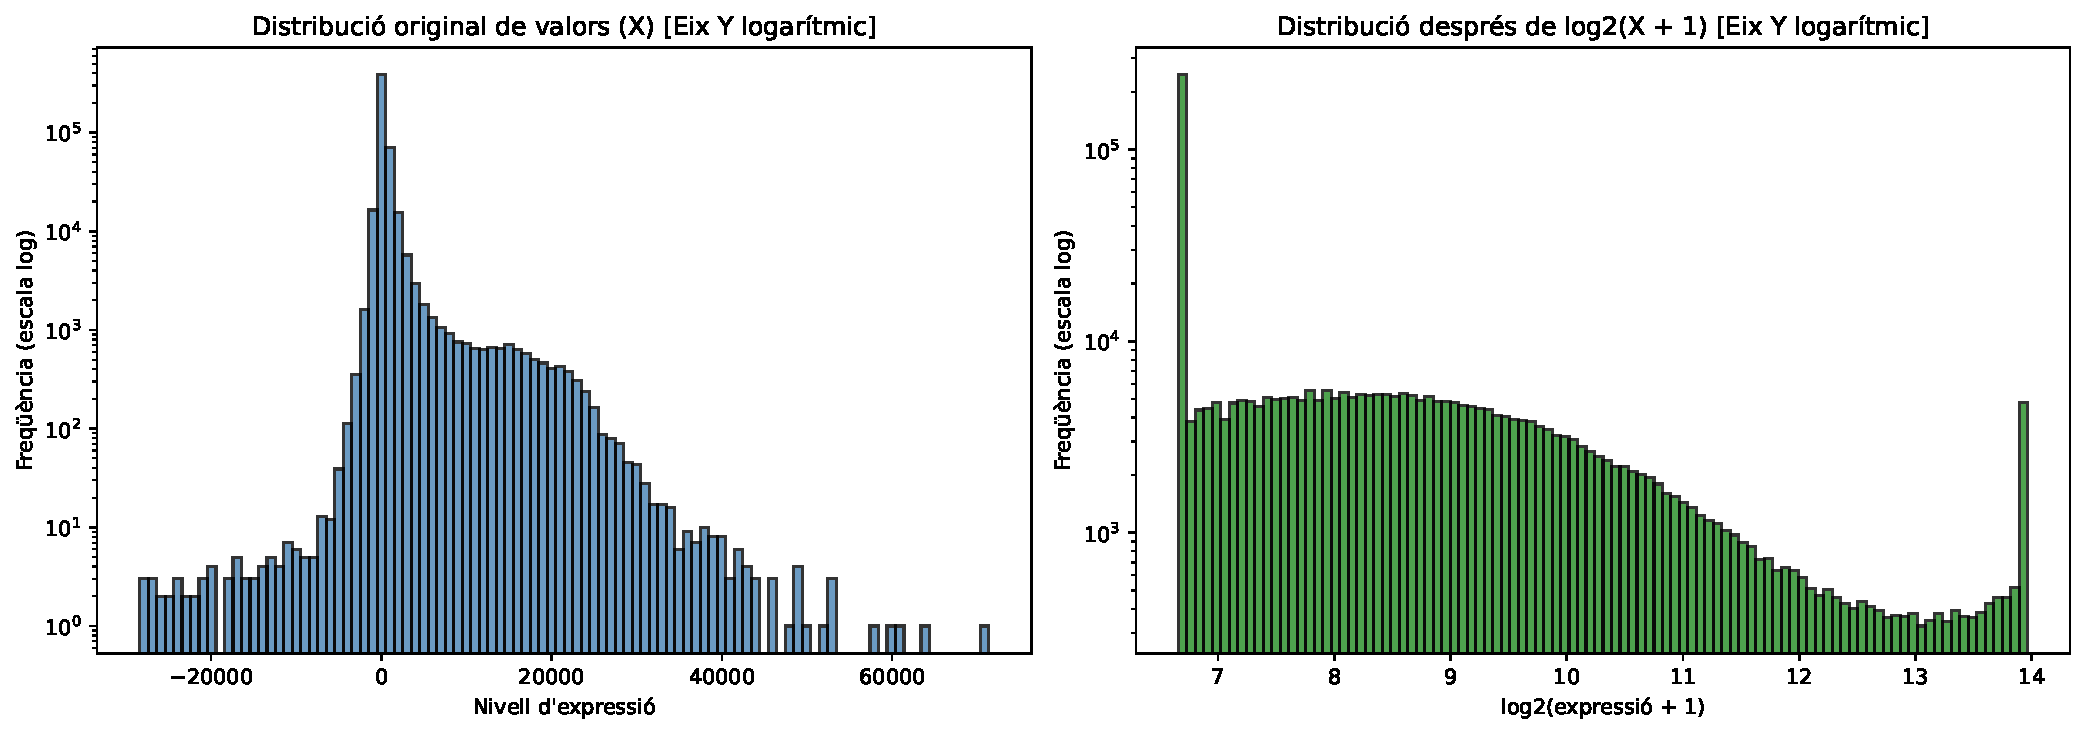
\includegraphics[width=0.95\textwidth]{hist_log.pdf}
\caption{Distribució de les intensitats d'expressió abans (esquerra) i després (dreta) del retall a $[100,16000]$ i de la transformació $\log_2(x+1)$. L'eix vertical és logarítmic.}
\label{fig:hist}
\end{figure}

La Taula~\ref{tab:comparacio} resumeix els quatre mètodes sobre els 72 pacients i la Figura~\ref{fig:dendro} mostra el dendrograma de l'enllaç \emph{average}.

\begin{table}[!htb]
\centering
\begin{tabular}{llcc}
\toprule
Mètode & Distància & Mides dels 2 grups & ARI \\
\midrule
Single   & correlació & [71, 1]  & $-0{,}013$ \\
Complete & correlació & [29, 43] & 0,787 \\
Average  & correlació & [31, 41] & 0,690 \\
K-Means  & euclidiana & --       & \textbf{0,890} \\
\bottomrule
\end{tabular}
\caption{Comparació de mètodes per a $k=2$ (mides reals: 47 ALL i 25 AML). En negreta, l'ARI màxim (K-Means).}
\label{tab:comparacio}
\end{table}

\begin{itemize}
  \item \textbf{Single} falla: separa un únic pacient i deixa la resta junta (ARI $\approx0$) per l'efecte cadena.
  \item \textbf{Complete} té el millor ARI entre els jeràrquics (0,787), per sobre de 0,7.
  \item \textbf{Average}, l'enllaç triat per al dendrograma i el clustermap, queda just per sota (0,690): l'enllaç condiciona el resultat.
\end{itemize}
Cap partició té mides 47/25, així que cap recupera exactament el diagnòstic; tanmateix, \textbf{K-Means} és la que s'hi acosta més (ARI 0,890).

\begin{figure}[!htb]
\centering
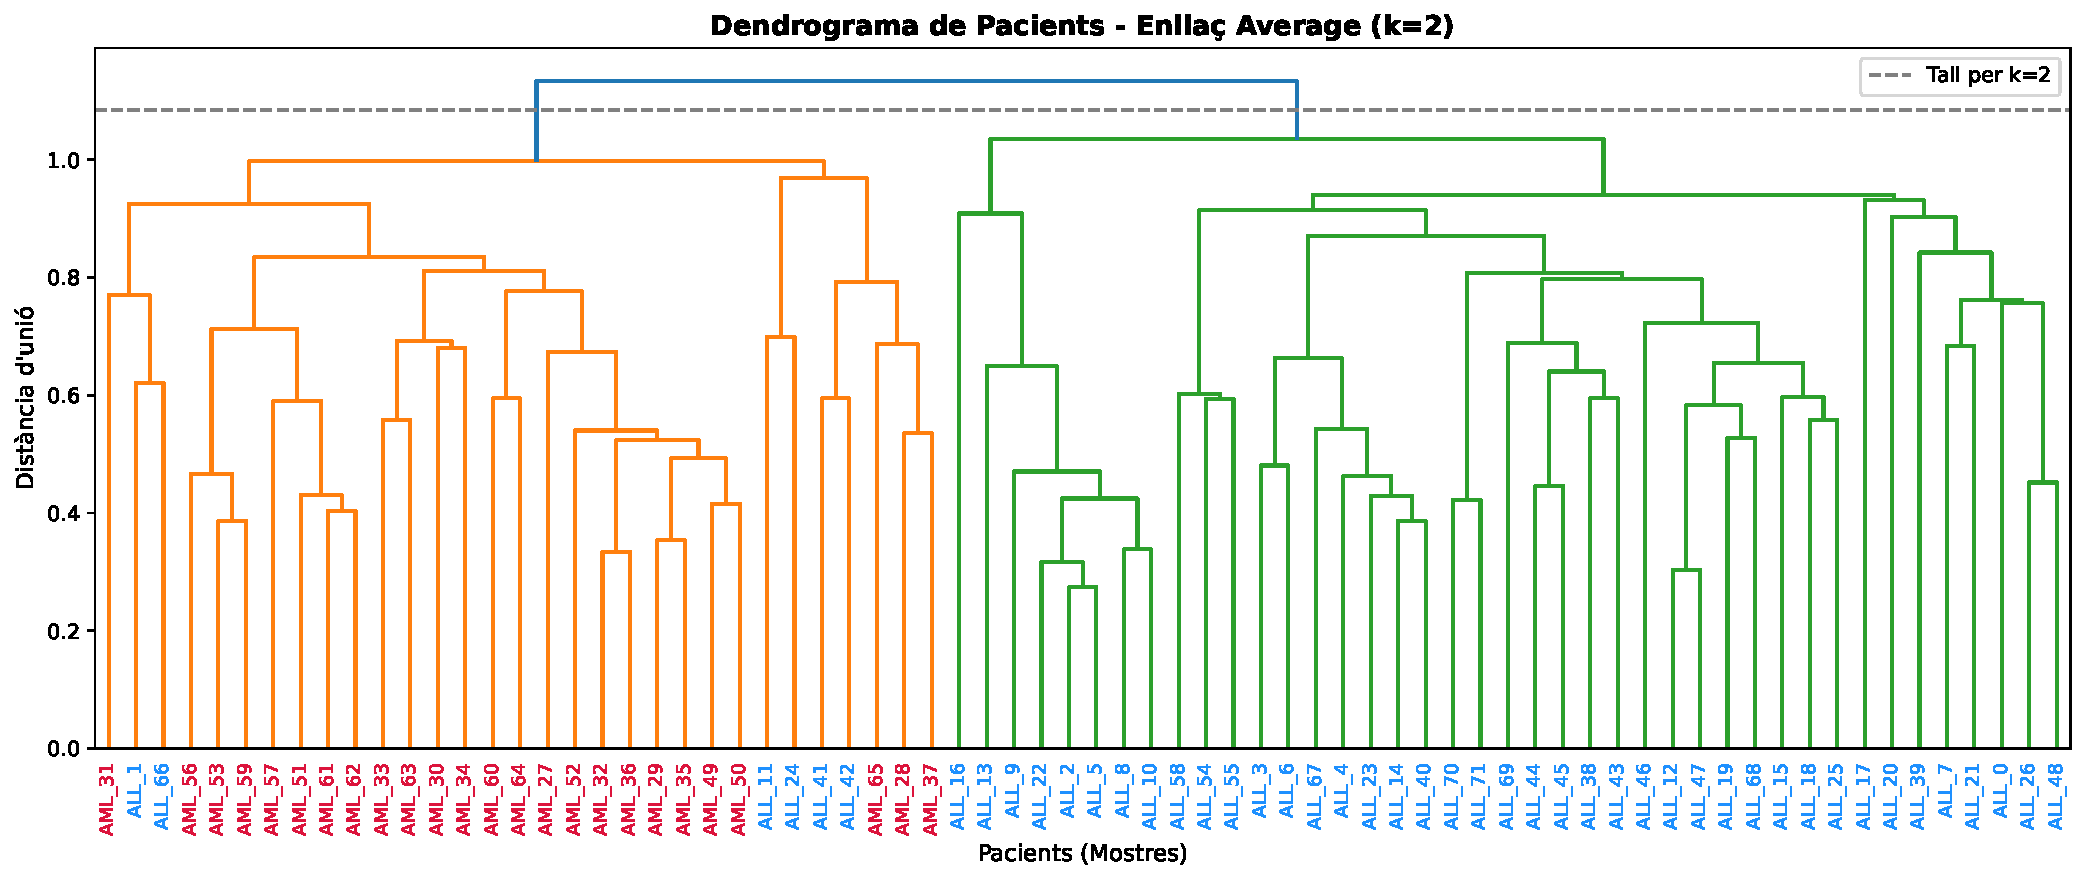
\includegraphics[width=\textwidth]{dendrograma_pacients_average.pdf}
\caption{Dendrograma dels 72 pacients (enllaç \emph{average}, distància de correlació). Les etiquetes són blaves per a ALL i vermelles per a AML; la línia grisa discontínua és el tall a $k=2$.}
\label{fig:dendro}
\end{figure}

Pel que fa a K-Means (Figura~\ref{fig:kmeans}), la inèrcia baixa de manera contínua (de 30.821 a $k=2$ fins a 22.841 a $k=8$) i no mostra un colze clar, de manera que el mètode del colze no ajuda a triar $k$. La silueta, en canvi, és màxima a $k=2$ (0,1352) i decreix fins a 0,0683 a $k=8$, la qual cosa coincideix amb els dos diagnòstics reals. Els valors són baixos (inferiors a 0,14): els grups són reconeixibles però no estan gaire separats en un espai de 500 dimensions.

\begin{figure}[!htb]
\centering
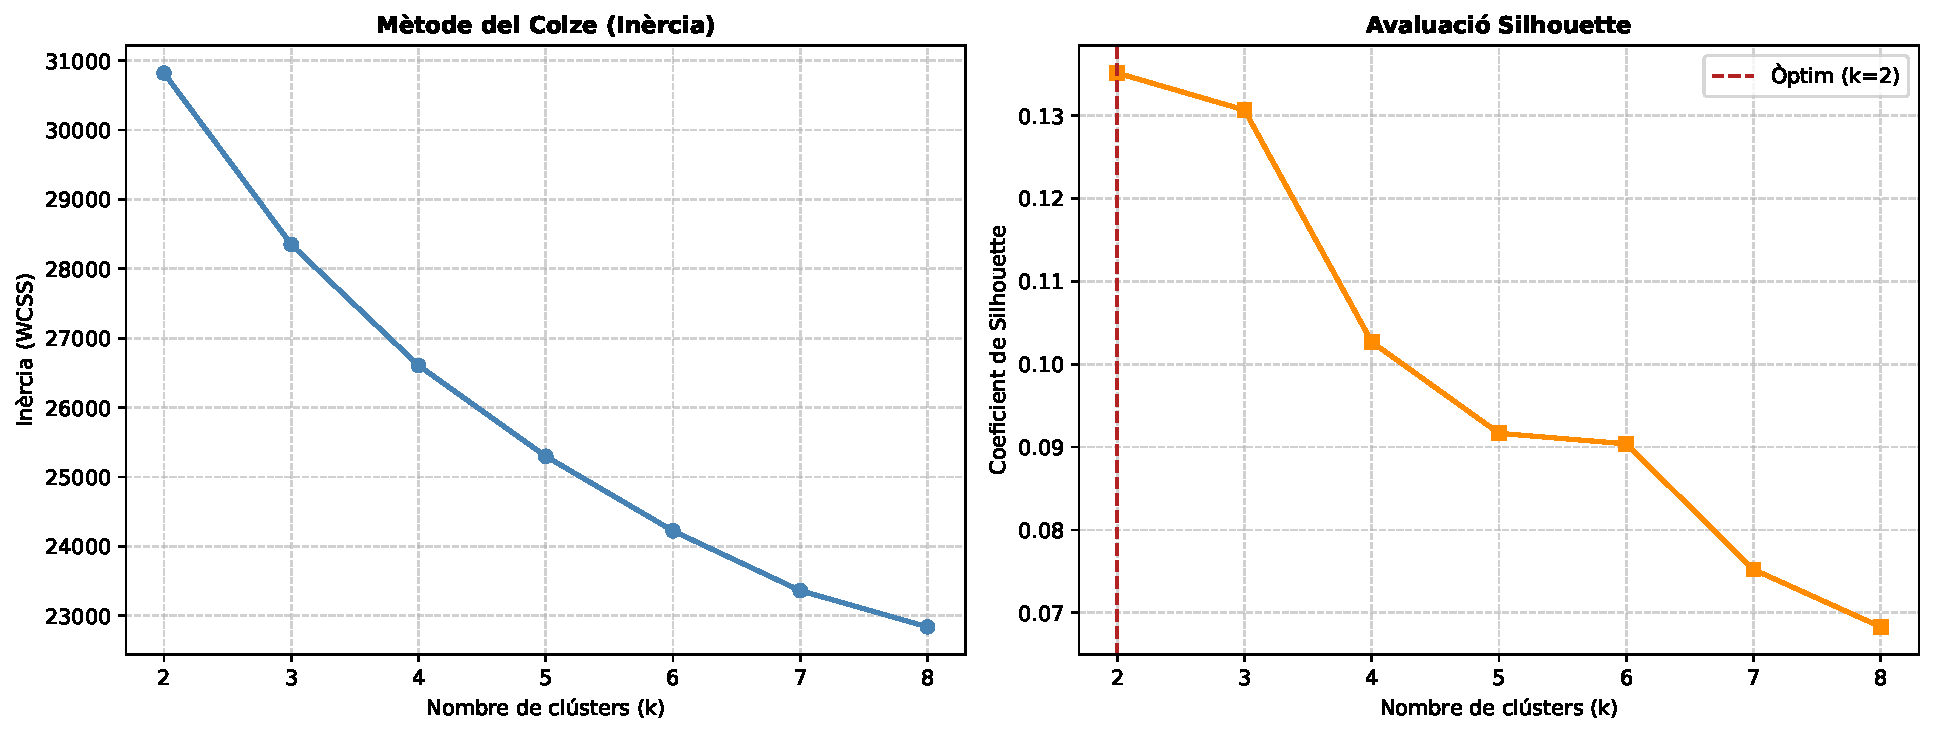
\includegraphics[width=\textwidth]{kmeans_pacients_colze_silhouette.pdf}
\caption{Mètode del colze (esquerra) i coeficient de Silhouette (dreta) per a K-Means.}
\label{fig:kmeans}
\end{figure}

Per als mòduls de gens (Taula~\ref{tab:moduls}), la silueta és màxima per a $k=2$ (0,1812), amb dos mòduls de 178 i 322 gens. Per a $k$ més gran apareixen mòduls molt petits (de 3, 4 o 7 gens) i la silueta empitjora, tot i que té un màxim local a $k=10$ (0,1394), que donaria una partició més fina. Es manté $k=2$ per criteri de silueta; és una divisió gruixuda que informa de dos grans patrons d'expressió i no de mòduls funcionals concrets.

\begin{table}[!htb]
\centering\small
\begin{tabular}{cc>{\raggedright\arraybackslash}p{7cm}}
\toprule
$k$ & Silueta & Mides dels mòduls \\
\midrule
2  & \textbf{0,1812} & 178, 322 \\
3  & 0,1302 & 178, 7, 315 \\
4  & 0,1188 & 178, 7, 278, 37 \\
5  & 0,1088 & 178, 7, 278, 15, 22 \\
6  & 0,1125 & 49, 129, 7, 278, 15, 22 \\
7  & 0,0929 & 49, 129, 3, 4, 278, 15, 22 \\
8  & 0,1297 & 49, 129, 3, 4, 159, 119, 15, 22 \\
9  & 0,1276 & 49, 129, 3, 4, 159, 119, 15, 4, 18 \\
10 & 0,1394 & 49, 129, 3, 4, 159, 27, 92, 15, 4, 18 \\
\bottomrule
\end{tabular}
\caption{Silueta i mida dels mòduls de gens per a cada $k$ (enllaç \emph{average}, distància de correlació).}
\label{tab:moduls}
\end{table}

Per entendre què aporta el clustering, la Figura~\ref{fig:heat_a} mostra la matriu $X_{\text{clean}}$ sense reordenar: columnes en l'ordre original dels pacients i files en l'ordre de selecció dels gens (de variància creixent). Cada cel·la és el z-score d'un gen en un pacient (vermell: expressió per sobre de la mitjana d'aquell gen; blau: per sota). En aquest ordre no hi ha cap criteri que agrupi gens o pacients semblants i els patrons no es poden llegir. La Figura~\ref{fig:heat_b} mostra la mateixa matriu reordenada pels dos dendrogrames: els valors no canvien, només l'ordre, i els gens i pacients amb perfils semblants queden adjacents. Així apareixen blocs de color i les barres de diagnòstic i de mòdul s'agrupen en trams contigus. Es veu que els pacients AML estan gairebé ben separats, ja que la majoria formen un bloc contigu, i a simple vista el mòdul~2 sembla més expressat en els AML i el mòdul~1 en molts dels ALL.

\begin{figure}[!htb]
\centering
\begin{subfigure}[t]{0.49\textwidth}
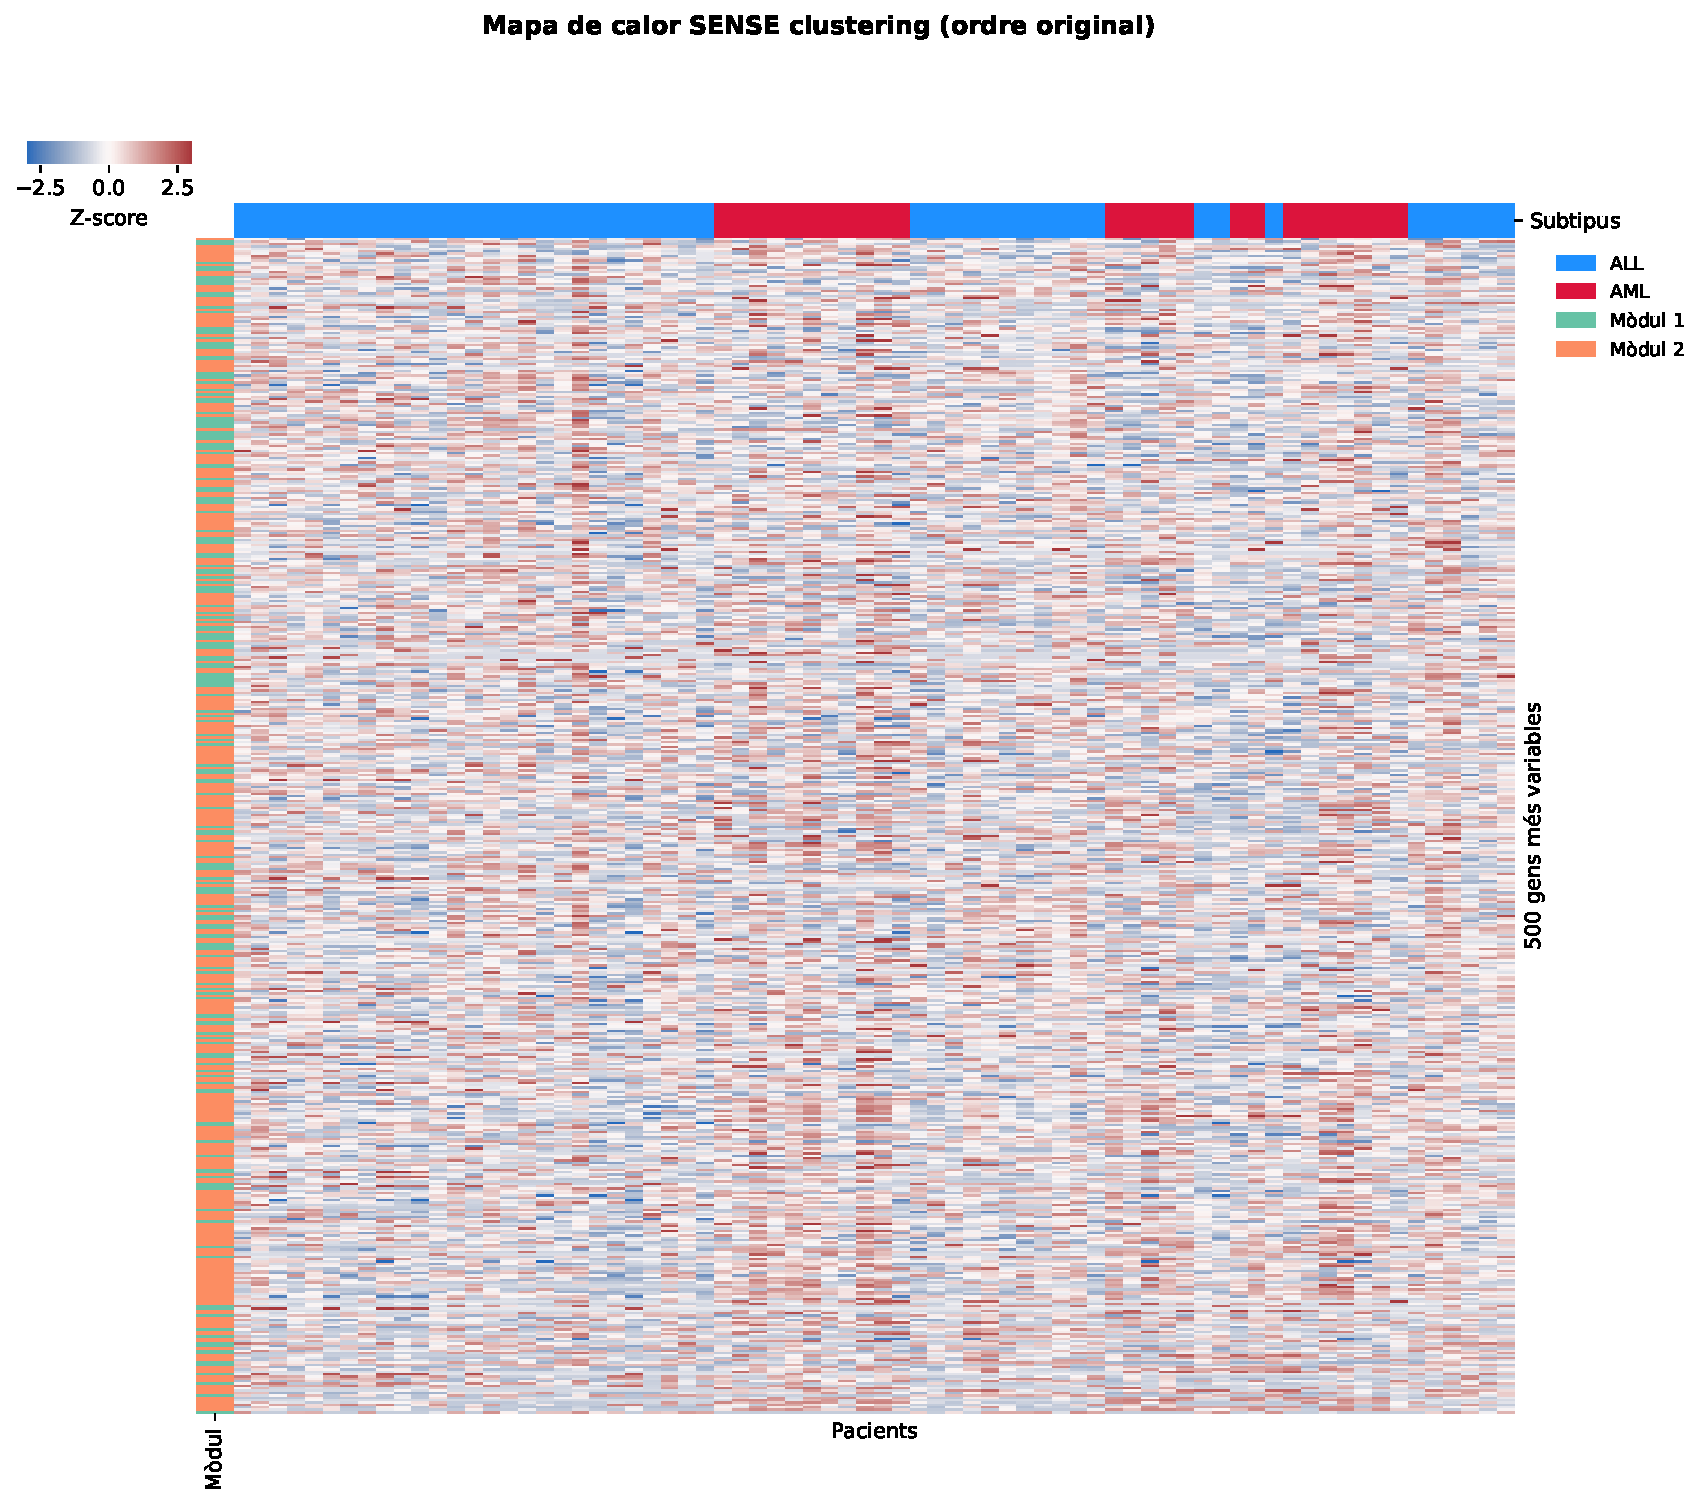
\includegraphics[width=\textwidth]{heatmap_sense_clustering.pdf}
\caption{Sense clustering.}
\label{fig:heat_a}
\end{subfigure}\hfill
\begin{subfigure}[t]{0.49\textwidth}
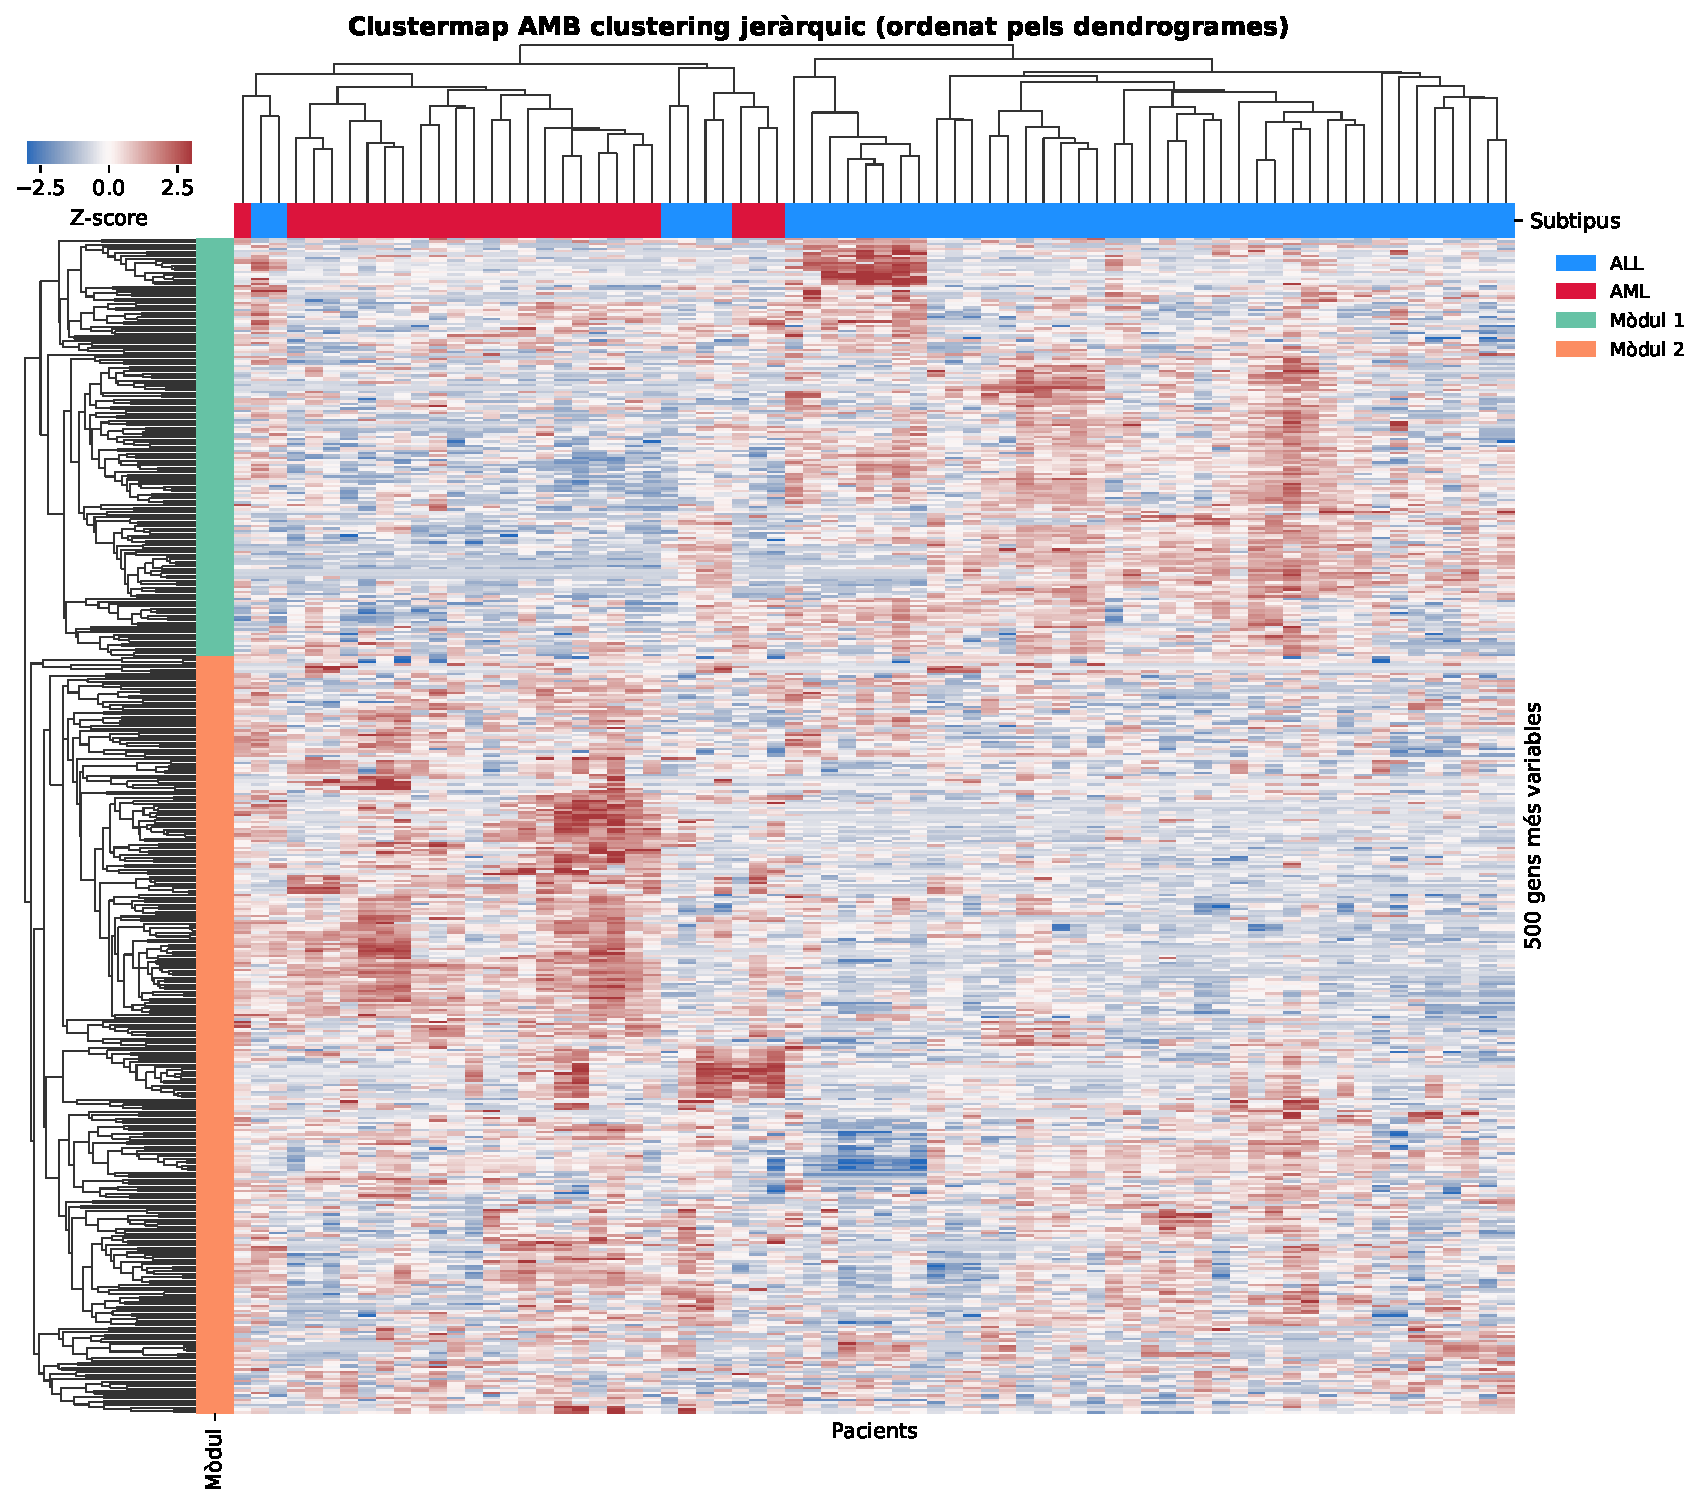
\includegraphics[width=\textwidth]{clustermap_expressio.pdf}
\caption{Amb clustering jeràrquic.}
\label{fig:heat_b}
\end{subfigure}
\caption{Z-score dels 500 gens més variables en els 72 pacients, sense reordenar (a) i reordenat pels dendrogrames de gens i pacients, enllaç \emph{average} (b). Barres de color: diagnòstic (ALL blau, AML vermell) i mòdul de gens.}
\label{fig:heatmap}
\end{figure}

%====================================================================
\vspace{0.4cm}
\section{Limitacions}

Primer, l'alta dimensionalitat: amb 500 característiques i només 72 pacients, les distàncies tendeixen a concentrar-se i la silueta és baixa (0,14--0,18) encara que els grups coincideixin amb el diagnòstic. Segon, la sensibilitat al preprocessament: el retall, la selecció de 500 gens i el logaritme afecten els resultats i no s'ha fet una anàlisi de sensibilitat sistemàtica (per exemple, amb 100, 500 i 1.000 gens). Tercer, el tall a $k=2$: l'ARI es calcula amb el nombre de diagnòstics coneguts i, per als jeràrquics, aquest valor és una decisió prèvia (la silueta de K-Means també indica $k=2$). Quart, per als mòduls de gens s'ha usat directament \emph{average}, sense comparar-lo amb la resta d'enllaços.

A més, es treballa amb un sol conjunt de dades petit, amb mostres de diversos hospitals, de manera que el clustering podria no distingir els efectes de laboratori del senyal biològic. Els mòduls no s'han anotat biològicament i, per tant, no es pot afirmar que tinguin significat funcional. Tampoc s'ha fet cap detecció d'anomalies, així que el pacient aïllat per \emph{single} no s'ha analitzat; queda pendent per a una possible continuació del projecte.


\vspace{0.4cm}
\section{Conclusions}

Els resultats permeten respondre els quatre objectius. Sense usar etiquetes, K-Means (ARI 0,890) i l'enllaç \emph{complete} (0,787) superen l'ARI de 0,7 plantejat i recuperen en gran part la distinció ALL/AML, mentre que \emph{average} (0,690) hi queda just per sota; cap partició, però, reprodueix exactament els grups 47/25. La comparació de mètodes mostra que l'enllaç condiciona el resultat: \emph{single} falla per l'efecte cadena i \emph{complete} i \emph{average} donen ARI diferents, de manera que convé validar amb una mètrica externa quan n'hi ha. Pel que fa als gens, la silueta en tria dos mòduls (178 i 322), una divisió gruixuda i de silueta baixa que no equival a mòduls funcionals, de manera que aquest objectiu s'assoleix només en part. Finalment, el clustermap integra gens i pacients amb els diagnòstics i els mòduls, i mostra què aporta el clustering respecte del mapa de calor brut. En conjunt, l'aprenentatge no supervisat, amb un preprocessament acurat i una distància adequada, recupera bona part de l'estructura biològica sense usar les etiquetes. Com a línies de millora es plantegen una anàlisi de sensibilitat al nombre de gens i al preprocessament, la detecció d'anomalies (Isolation Forest), la comparació amb DBSCAN i models de mescla gaussiana, l'anotació biològica dels mòduls i la repetició de l'estudi amb dades de seqüenciació d'ARN, que requereixen un preprocessament diferent.

%====================================================================
\vspace{0.4cm}
\begin{thebibliography}{9}
\bibitem{golub} Golub, T. R. et al. (1999). Molecular classification of cancer: class discovery and class prediction by gene expression monitoring. \textit{Science}, 286(5439), 531--537.
\bibitem{eisen} Eisen, M. B., Spellman, P. T., Brown, P. O., Botstein, D. (1998). Cluster analysis and display of genome-wide expression patterns. \textit{PNAS}, 95(25), 14863--14868.
\bibitem{rousseeuw} Rousseeuw, P. J. (1987). Silhouettes: a graphical aid to the interpretation and validation of cluster analysis. \textit{Journal of Computational and Applied Mathematics}, 20, 53--65.
\bibitem{hubert} Hubert, L., Arabie, P. (1985). Comparing partitions. \textit{Journal of Classification}, 2, 193--218.
\bibitem{sklearn} Pedregosa, F. et al. (2011). Scikit-learn: machine learning in Python. \textit{Journal of Machine Learning Research}, 12, 2825--2830.
\end{thebibliography}

%====================================================================
\appendix
\vspace{0.4cm}
\section{Fórmules complementàries}
\label{ann:formules}
\small

\textbf{K-Means.} Minimitza la inèrcia $J=\sum_{j=1}^{k}\sum_{x\in C_j}\lVert x-\mu_j\rVert^2$ alternant dos passos fins que res canvia: assignar cada punt al centre més proper i recalcular cada centre com la mitjana dels seus punts.

\textbf{Adjusted Rand Index.} Sigui $n_{ij}$ el nombre de pacients que són al grup $i$ de la partició trobada i a la classe $j$ del diagnòstic, amb sumes per files $a_i$ i per columnes $b_j$, i $n$ el total. Llavors
\[
\mathrm{ARI}=\frac{\sum_{ij}\binom{n_{ij}}{2}-\Big[\sum_i\binom{a_i}{2}\sum_j\binom{b_j}{2}\Big]\Big/\binom{n}{2}}
{\tfrac12\Big[\sum_i\binom{a_i}{2}+\sum_j\binom{b_j}{2}\Big]-\Big[\sum_i\binom{a_i}{2}\sum_j\binom{b_j}{2}\Big]\Big/\binom{n}{2}}.
\]
\end{document}
